\documentclass[tikz,border=10pt]{standalone}
\usepackage{tikz}
\usepackage{amssymb}
\usetikzlibrary{shapes.geometric, arrows.meta, positioning, calc, backgrounds, fit}

\definecolor{pbblue}{HTML}{EBF5FB}
\definecolor{pbdarkblue}{HTML}{1B4F72}
\definecolor{pbmint}{HTML}{E8F8F5}
\definecolor{pbdarkgreen}{HTML}{0E6251}
\definecolor{pblavender}{HTML}{F4ECF7}
\definecolor{pbdarkpurple}{HTML}{512E5F}
\definecolor{pbyellow}{HTML}{FEF9E7}
\definecolor{pbdarkyellow}{HTML}{7D6608}
\definecolor{pbcoral}{HTML}{FDEDEC}
\definecolor{pbdarkred}{HTML}{78281F}
\definecolor{pbgray}{HTML}{F8F9F9}

\begin{document}
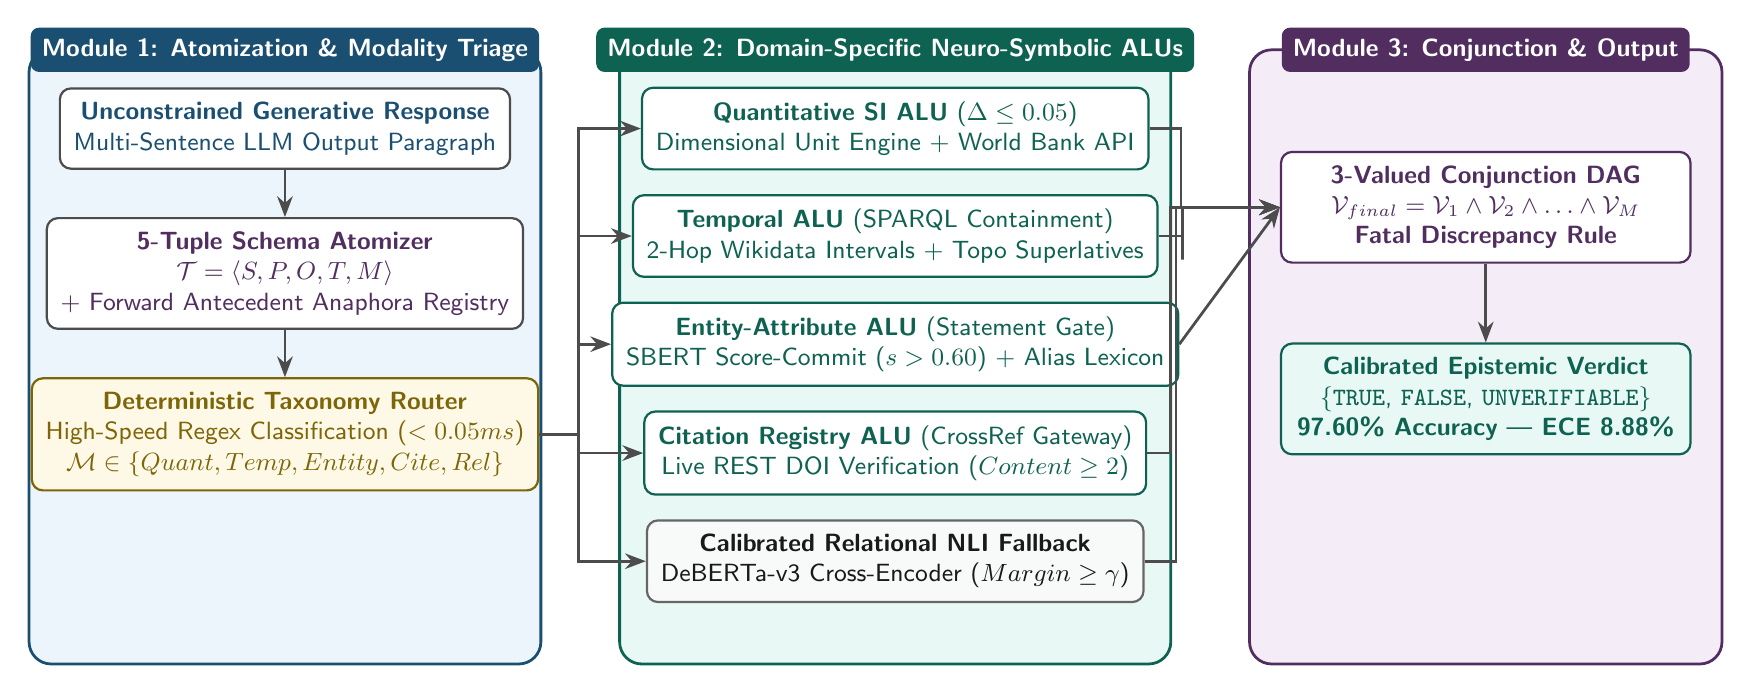
\begin{tikzpicture}[
    font=\sffamily\small,
    box/.style={draw=black!70, rounded corners=4pt, line width=0.8pt, align=center, inner sep=5pt},
    arrow/.style={-{Stealth[scale=1.0]}, line width=1.0pt, draw=black!70}
]

% ==================== MODULE 1: Atomization & Routing ====================
\draw[fill=pbblue, draw=pbdarkblue, rounded corners=8pt, line width=1pt] (-0.3, -4.6) rectangle (6.2, 3.2);
\node[fill=pbdarkblue, text=white, font=\bfseries\sffamily\small, rounded corners=3pt, inner sep=4pt] at (2.95, 3.2) {Module 1: Atomization \& Modality Triage};

\node[box, fill=white, text=pbdarkblue, minimum width=5.6cm] (m1_input) at (2.95, 2.2) {\textbf{Unconstrained Generative Response}\\Multi-Sentence LLM Output Paragraph};

\node[box, fill=white, text=pbdarkpurple, minimum width=5.6cm, below=0.6cm of m1_input] (m1_atom) {\textbf{5-Tuple Schema Atomizer}\\$\mathcal{T} = \langle S, P, O, T, M \rangle$\\+ Forward Antecedent Anaphora Registry};

\node[box, fill=pbyellow, draw=pbdarkyellow, text=pbdarkyellow, minimum width=5.6cm, below=0.6cm of m1_atom] (m1_router) {\textbf{Deterministic Taxonomy Router}\\High-Speed Regex Classification ($< 0.05\text{ms}$)\\$\mathcal{M} \in \{\text{Quant}, \text{Temp}, \text{Entity}, \text{Cite}, \text{Rel}\}$};

\draw[arrow] (m1_input) -- (m1_atom);
\draw[arrow] (m1_atom) -- (m1_router);

% ==================== MODULE 2: Specialized ALU Suite ====================
\draw[fill=pbmint, draw=pbdarkgreen, rounded corners=8pt, line width=1pt] (7.2, -4.6) rectangle (14.2, 3.2);
\node[fill=pbdarkgreen, text=white, font=\bfseries\sffamily\small, rounded corners=3pt, inner sep=4pt] at (10.7, 3.2) {Module 2: Domain-Specific Neuro-Symbolic ALUs};

\node[box, fill=white, draw=pbdarkgreen, text=pbdarkgreen, minimum width=6.2cm] (alu_q) at (10.7, 2.2) {\textbf{Quantitative SI ALU} ($\Delta \le 0.05$)\\Dimensional Unit Engine + World Bank API};

\node[box, fill=white, draw=pbdarkgreen, text=pbdarkgreen, minimum width=6.2cm, below=0.3cm of alu_q] (alu_t) {\textbf{Temporal ALU} (SPARQL Containment)\\2-Hop Wikidata Intervals + Topo Superlatives};

\node[box, fill=white, draw=pbdarkgreen, text=pbdarkgreen, minimum width=6.2cm, below=0.3cm of alu_t] (alu_e) {\textbf{Entity-Attribute ALU} (Statement Gate)\\SBERT Score-Commit ($s > 0.60$) + Alias Lexicon};

\node[box, fill=white, draw=pbdarkgreen, text=pbdarkgreen, minimum width=6.2cm, below=0.3cm of alu_e] (alu_c) {\textbf{Citation Registry ALU} (CrossRef Gateway)\\Live REST DOI Verification ($\text{Content} \ge 2$)};

\node[box, fill=pbgray, draw=black!60, text=black!90, minimum width=6.2cm, below=0.3cm of alu_c] (alu_r) {\textbf{Calibrated Relational NLI Fallback}\\DeBERTa-v3 Cross-Encoder ($\text{Margin} \ge \gamma$)};

% Connect Router to ALUs
\draw[arrow] (m1_router.east) -- ++(0.5,0) |- (alu_q.west);
\draw[arrow] (m1_router.east) -- ++(0.5,0) |- (alu_t.west);
\draw[arrow] (m1_router.east) -- ++(0.5,0) |- (alu_e.west);
\draw[arrow] (m1_router.east) -- ++(0.5,0) |- (alu_c.west);
\draw[arrow] (m1_router.east) -- ++(0.5,0) |- (alu_r.west);

% ==================== MODULE 3: Conjunction & Decision ====================
\draw[fill=pblavender, draw=pbdarkpurple, rounded corners=8pt, line width=1pt] (15.2, -4.6) rectangle (21.2, 3.2);
\node[fill=pbdarkpurple, text=white, font=\bfseries\sffamily\small, rounded corners=3pt, inner sep=4pt] at (18.2, 3.2) {Module 3: Conjunction \& Output};

\node[box, fill=white, draw=pbdarkpurple, text=pbdarkpurple, minimum width=5.2cm] (dag) at (18.2, 1.2) {\textbf{3-Valued Conjunction DAG}\\$\mathcal{V}_{\text{final}} = \mathcal{V}_1 \wedge \mathcal{V}_2 \wedge \dots \wedge \mathcal{V}_M$\\\textbf{Fatal Discrepancy Rule}};

\node[box, fill=pbmint, draw=pbdarkgreen, text=pbdarkgreen, minimum width=5.2cm, below=1.0cm of dag] (decision) {\textbf{Calibrated Epistemic Verdict}\\\{\texttt{TRUE}, \texttt{FALSE}, \texttt{UNVERIFIABLE}\}\\\textbf{97.60\% Accuracy} | \textbf{ECE 8.88\%}};

\draw[arrow] (alu_q.east) -| ++(0.4,-0.6) |- (dag.west);
\draw[arrow] (alu_t.east) -| ++(0.3,-0.3) |- (dag.west);
\draw[arrow] (alu_e.east) -- (dag.west);
\draw[arrow] (alu_c.east) -| ++(0.3,0.3) |- (dag.west);
\draw[arrow] (alu_r.east) -| ++(0.4,0.6) |- (dag.west);
\draw[arrow] (dag) -- (decision);

\end{tikzpicture}
\end{document}